\documentclass[10pt, fullpage, a4paper, titlepage]{article}
\usepackage{graphicx, latexsym}
\usepackage{setspace}
\usepackage{apalike}
\usepackage{amssymb, amsmath, amsthm}
\usepackage{bm}
\usepackage{epstopdf}
\usepackage[]{hyperref}
\usepackage{caption}
\usepackage{subcaption}
\usepackage{xcolor}

\title{MLaRPIS Homework Exercise 1}
\author{Pepijn Vink}
\date{\today}
\pagecolor{white}

\begin{document}
\maketitle
\newpage

\section{Bayes Rule}
Bayes Rule is a formula that is used to update the prior using the likelihood to obtain the posterior distribution.
\subsection{Equation}
This is the equation for Bayes rule.
\begin{equation}
    P( \theta|D ) = \frac{P(D|\theta) P(\theta)}{P(D)} = \frac{P(D|\theta) P(\theta)}{\int P(D | \theta) P(\theta) d\theta} 
\end{equation}
\subsection{Visualizations}
\begin{figure}[h]
\centering
\begin{subfigure}{0.4\linewidth}
\centering

\includegraphics[width = \linewidth]{histogram.png}
\caption{Histogram}
\end{subfigure}
\hfill
\begin{subfigure}{0.4\linewidth}
\centering

\includegraphics[width = \linewidth]{density.png}
\caption{Densityplot}
\end{subfigure}
\hfill
\begin{subfigure}{0.4\linewidth}
\centering

\includegraphics[width = \linewidth]{stripplot.png}
\caption{Stripplot}
\end{subfigure}
\hfill
\begin{subfigure}{0.4\linewidth}
\centering
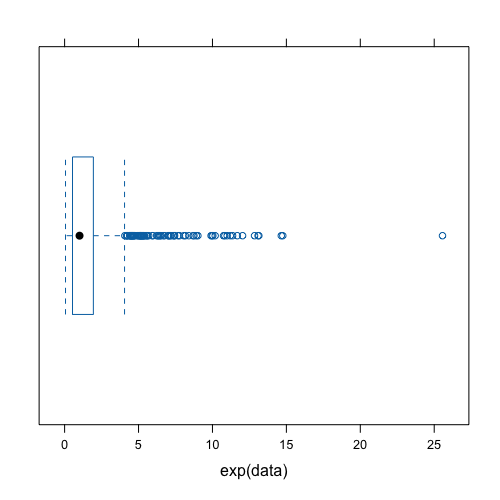
\includegraphics[width = \linewidth]{bwplot.png}
\caption{Boxplot}
\end{subfigure}
\caption{Different plots of the same data, sometimes transformed. No particular objective other than it being an exercise.}
\end{figure}
% latex table generated in R 4.2.1 by xtable 1.8-4 package
% Wed Sep 13 18:36:45 2023
\begin{table}[ht]
\caption{The same data, but now in a table. Only the first nine rows are displayed.}
\centering
\begin{tabular}{rrrrr}
  \hline
 & data & squared1 & squared2 & exponent \\ 
  \hline
1 & -0.56 & 0.31 & 0.31 & 0.57 \\ 
  2 & -0.23 & 0.05 & 0.05 & 0.79 \\ 
  3 & 1.56 & 2.43 & 2.43 & 4.75 \\ 
  4 & 0.07 & 0.00 & 0.00 & 1.07 \\ 
  5 & 0.13 & 0.02 & 0.02 & 1.14 \\ 
  6 & 1.72 & 2.94 & 2.94 & 5.56 \\ 
  7 & 0.46 & 0.21 & 0.21 & 1.59 \\ 
  8 & -1.27 & 1.60 & 1.60 & 0.28 \\ 
  9 & -0.69 & 0.47 & 0.47 & 0.50 \\ 
   \hline
\end{tabular}
\end{table}
\subsection{Story}
The Enchanted Garden and the Magical Dove\

Once, in a land covered by mists and whispers, there lay an enchanting garden hidden behind a great stone wall. No one knew who had built the wall or why, but one thing was for certain – nobody had ever seen what was behind it.\

A little boy named Peter lived in a village nearby. Fuelled by curiosity and tales of magical creatures, he often dreamt of the wonders that the walled garden might hold. One day, unable to resist its lure any longer, he decided to find a way in.\

As he approached the towering stone barrier, he noticed a tiny gap just big enough for him to peek through. The garden inside was bathed in a shimmering golden light, unlike any he had ever seen. To his amazement, in the center stood a magnificent tree with leaves that glittered as if they were made of starlight. And resting on one of its branches was a dove, glowing with the same luminous hue.\

Before he could process this beautiful sight, the dove spoke to his in a voice as soft as the wind, "To enter the garden, one must share a pure and selfless desire."\

Peter, with his heart pounding, whispered his wish, "I wish for everyone in my village to be happy and free from suffering."\

The massive stone door, seemingly of its own accord, began to open. The luminous dove flew to Peter and rested on his shoulder. "Your wish is genuine, and so you may enter," it said.\

Inside, the garden was more wondrous than Peter had ever imagined. Flowers sang in soft harmonies, and a gentle breeze carried the sweetest of fragrances. Every step he took made the grass shimmer with colors she'd never seen before.\

The dove explained that this was an Enchanted Garden, a place where one’s purest wishes could come true. But, there was a catch. To make his wish a reality, Peter had to plant a seed from the magical tree in his village and care for it with unwavering love and dedication.\

Peter accepted the challenge. With the seed safely tucked in his pocket and the dove guiding her, he returned to his village.\

Years went by, and with Peter's love, the seed grew into a magnificent tree, similar to the one in the Enchanted Garden. With its growth, joy and happiness blossomed in the village like never before.\

And so, in a village once shadowed by mystery, there stood a tree that bore witness to the pure heart of a boy and his luminous companion, reminding everyone that magic was always just a wish away.\
\end{document}